\section{Introduction}
\label{sec:linked_data} 

In recent years, the amount of Linked Data on the Web has been
increasing rapidly. This is largely due to community efforts such as
the Linking Open Data project, and increasing interests of enterprises
and governments. Datasets made publicly available on the Web as Linked
Data cover different domains, including life sciences (e.g. DrugBank,
UniProt, PubMed), geographic locations (e.g. World Factbook, Geo Names), media and entertainment (MusicBrainz, Last.FM, BBC
Programmes). There are also cross-domain encyclopedic datasets such as
Freebase and DBpedia (the structured data counterpart of
Wikipedia). Besides enterprises, such as media companies like BBC and
Last.FM, many governments (e.g. US, UK) recently started to make data
of public interest available to citizens, including CO2, Mortality,
Energy and Postcodes. We refer to the public
Website~\footnote{\url{http://linkeddata.org/}} for an overview of
concepts, activities, projects, and datasets related to Linked Data.

Aiming at making Linked Data available to
data-intensive processes and Web users, researchers recently started
to study the problem of Linked Data query
processing~\cite{hartig_executing_2009,harth_data_2010,ladwig_linked_2010,hartig_zero_2011,sihjoin_2011}. Just
like Web pages, Linked Data on the Web are accessible through URI
lookups. According to the Linked Data principles
\cite{bizer_linked_2009}, dereferencing a Linked Data URI via HTTP
should return a machine-readable description (usually in RDF) of the
entity identified by the URI. Each URI therefore represents a virtual
``data source''.

Figs.~\ref{fig:sources} \& \ref{fig:query} show examples of Linked
Data sources with their data and a Linked Data query,
respectively. For processing such a query, Linked Data sources to be used may not be stored or cached locally, but
are retrieved at run-time via dereferencing the URIs mentioned in the sources. In this way,
Linked Data query processing specifically aim to deal with the rapidly evolving nature of
the Web of data and to deliver results that are always
up-to-date. In this example, the query engine may dereference the
URIs \emph{ex:beatles}, \emph{ex:sgt\_pepper} and \emph{ex:lucy} to
produce the result \emph{``Lucy...''} for the query variable
$?name$.
% \dtr{need example which illustrate what is linked
%   data query processing, and why it is really useful, e.g. freshness
%   of results important due fast update rates of data, what else?}

Thus, processing structured queries against Linked Data can be seen as
a special case of federated query processing. However, the restricted
access pattern based on HTTP lookup and the highly distributed nature
of Linked Data sources resulting from it, present unique challenges:

\begin{figure*}[ht]
  \centering
  \begin{minipage}{0.32\linewidth}
\begin{lstlisting}[breaklines=true,language=ttl,linewidth=0.98\linewidth,frame=single,caption=http://example.org/beatles]
ex:beatles 
  foaf:name "The Beatles" ;
  ex:album ex:help ;
  ex:album ex:sgt_pepper  .
\end{lstlisting}
  \end{minipage}
  \begin{minipage}{0.32\linewidth}
\begin{lstlisting}[breaklines=true,language=ttl,linewidth=0.98\linewidth,frame=single,caption=http://example.org/help]
ex:help 
  foaf:name "Help!" ;
  ex:song ex:night ;
  ex:song ex:girl .
\end{lstlisting}
  \end{minipage}
  \begin{minipage}{0.32\linewidth}
\begin{lstlisting}[breaklines=true,language=ttl,linewidth=0.98\linewidth,frame=single,caption=http://example.org/sgt\_pepper]
ex:sgt_pepper
  foaf:name "Sgt. Pepper" ;
  ex:song ex:lucy ;
  ex:song ex:friends .
\end{lstlisting}
  \end{minipage}
  \begin{minipage}{0.32\linewidth}
\begin{lstlisting}[breaklines=false,language=ttl,frame=single,linewidth=0.98\linewidth,caption=http://example.org/girl]
ex:girl
  foaf:name "Another Girl" .

\end{lstlisting}
  \label{fig:example}
  \end{minipage}
  \begin{minipage}{0.32\linewidth}
\begin{lstlisting}[breaklines=true,language=ttl,frame=single,linewidth=0.98\linewidth,showlines=true,caption=http://example.org/night]
ex:night 
  foaf:name "The Night..." .
\end{lstlisting}
  \end{minipage}
  \begin{minipage}{0.32\linewidth}
\begin{lstlisting}[breaklines=true,language=ttl,frame=single,showlines=true,caption=http://example.org/lucy]
ex:lucy
  foaf:name "Lucy..." .
\end{lstlisting}
  \end{minipage}

  \caption{Example Linked Data sources. The prefix \emph{ex:} expands
    to ``http://example.org/''.}
  \label{fig:sources}
\end{figure*}

\begin{itemize}
\item \textbf{Large number of sources.} Since every URI can be
  considered as a source, the \emph{number of Linked Data sources}
  that have to be processed is potentially very large. Hundreds of
  sources of varying size may have to be retrieved for a single
  trivial query~\cite{ladwig_linked_2010}.

\item \textbf{High cost for source retrieval.} Typically, while basic
  source statistics have been assumed to exist (especially for sources
  that have been processed before~\cite{ladwig_linked_2010}), it is
  not practical or desirable to assume that all data is available
  locally. Processing queries in
  this distributed setting however requires Linked Data sources to be
  \emph{retrieved as a whole}. This is because as opposed to standard
  federated query processing, where remote sources are actually
  endpoints that provide structured querying capabilities, only HTTP
  lookups are possible here. That is, instead of retrieving partial
  answers that possibly match large parts of the queries, only whole
  sources matching the URIs mentioned in the queries can be
  obtained. As a result, processing Linked Data sources becomes a
  separate task, and due to its relative high cost, requires special
  treatment during query processing.
  %	Without these advanced querying capabilities, the impact of
  % selecting sources on overall query performance becomes more
  % pronounced as the overhead of source retrieval is much higher.

\item \textbf{Different, conflicting optimization criteria.}
  Typically, the optimization of queries is based on one single goal,
  namely to minimize the \emph{cost} for computing all results. The
  large number of potentially relevant sources and their high
  processing costs lead to long execution times such that \emph{result
    completeness} is often no longer affordable in practical
  usage. Thus, addressing this requirement has not been the main goal in
  previous work on Linked Data query
  processing~\cite{hartig_executing_2009,harth_data_2010,ladwig_linked_2010}, which
  employs various termination criteria such as a maximum number of
  retrieved sources \cite{harth_data_2010}, and strategies to select only the best few sources~\cite{ladwig_linked_2010}. 
%  In 
%  fact, completeness has
%  never been crucial on the Web but rather, the goal of Web search for
%  instance, is to obtain some (best) results in a given amount of
%  time. In other words, not only the cost of processing but also the
%  amount of results (\emph{output cardinality}) play a role. 
  Instead of assuming completeness and optimizing exclusively for cost, other 
  criteria such as relevance, quality and cardinality of results, and trustworthy of sources may be considered in the various Linked Data use cases that are
  possible. This is problematic because these criteria are not always
  complementary. For instance, there is an inherent trade-off between
  output cardinality and cost: To produce more results, we have to
  retrieve more sources, which in turn increases processing cost (and
  vice versa).
\end{itemize}

\emph{Federated databases} are able to process queries over data that
is managed by several networked database systems, either centralized
\cite{zsu_principles_2011} or in a distributed, peer-to-peer fashion
\cite{huebsch_architecture_2005}. Every node in this federated setting 
hosts its data, and provides structured querying
capabilities such that query processing in this setting breaks down to
finding the right nodes to execute part of the queries and merging
results. For optimization, the main strategy is to leverage the
capabilities of the nodes, i.e. pushing the processing to the nodes,
and to minimize cost for transferring data (partial results)
\cite{kossmann_iterative_2000,zsu_principles_2011}. In the case where
nodes provide materialized views, this problem amounts to finding the
cost-optimal composition of views
\cite{pottinger_minicon:_2001}. These solutions are not applicable to
our setting because instead of partial results and views, nodes return
entire sources. That is, they possess only one capability, namely
``source scan'' (we choose this term to make clear the analogy of HTTP
source lookup and table scan). More precisely, \emph{not the
  composition of views or joined results but the selection of source scans and processing the resulting sources are crucial tasks in this setting.}
%Standard query optimization can be adopted to produce an optimal query plan. 

% Further, as completeness is not required, not only the order but also
% the selection of sources is critical for query optimization.
Selecting relevant sources for a given query has been a topic in
data integration research. There, sources are described
not only by their content, but also by their capabilities, and
algorithms that efficiently perform \emph{source selection} by using
source characteristics to prune the search space have been
proposed~\cite{levy_querying_1996}. However, source selection is
performed as a separate step. Also decoupled from query optimization
are the source ranking strategies recently applied in Linked Data
query processing~\cite{harth_data_2010,ladwig_linked_2010}. Because
source selection is an essential part of query processing, this kind
of \emph{local optimization may lead to sub-optimal overall plans}.
%\cite{nie_joint_2001}.


Further, all these approaches \emph{optimize towards one single
  criterion} (cost) only.

\begin{figure}[ht]
  \centering
  \begin{minipage}{0.75\linewidth}
\begin{lstlisting}[language=ttl,numbers=left,escapeinside={(*@}{@*)}]
SELECT ?name WHERE {
  ex:beatles ex:album  ?album . (*@\label{query:q1}@*)
  ?album     ex:song   ?song . (*@\label{query:q2}@*)
  ?song      foaf:name ?name . (*@\label{query:q3}@*)
}
\end{lstlisting}
  \end{minipage}
  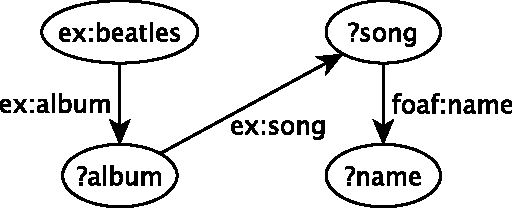
\includegraphics[width=0.7\linewidth]{figs/query-crop.pdf}
  \caption{Example query asking for names of songs in albums of the
    Beatles. The query consists of three triple patterns $q_1$ (line
    \ref{query:q1}), $q_2$ (line \ref{query:q2}), and $q_3$ (line
    \ref{query:q3}).}
  \label{fig:query}
\end{figure}

\textbf{Contributions.} Aiming at the challenges presented above, we
provide the following contributions:

\begin{itemize}
\item Solutions related to Linked Data query processing include Linked
  Data indexing~\cite{harth_data_2010}, query processing
  strategies~\cite{hartig_executing_2009,ladwig_linked_2010}, and
  using heuristics for adaptive ranking to select only the few best
  sources~\cite{ladwig_linked_2010}. However, to the best of our
  knowledge, this work is the \emph{first solution towards a
    systematic optimization of Linked Data query processing}.

\item In particular, we propose an optimization framework for Linked Data query processing, which incorporates
  \emph{both standard query operators} and \emph{source
    selection}. That is, we propose to extend the scope of query
  optimization from how to process data to which data to process. This
  is necessary to reflect the nature of Linked Data query processing,
  where source selection and scanning become an essential
  part. Further, this framework supports the \emph{joint optimization
    of several objectives}, cost and output cardinality in particular.

\item We propose a dynamic programming algorithm for the
  multi-objective optimization of this integrated process of source
  selection and query processing. It produces a set of Pareto-optimal
  query plans, which represent different trade-offs between optimization
  objectives.
  
\item After retrieval, sources can be re-used in different parts of
  the query. Essentially, this means that \emph{sharing of source
    scan operators} is possible. While this provides more room for
  optimization, it also makes dynamic programming technically more
  challenging: the cost function is no longer monotonic with regard to
  plan combination, which is due to the fact that the cost of subplans
  may vary, depending on the reusability of their sources. We provide
  \emph{tight bounds} for costs that take this effect into account.
\end{itemize}



% In this paper, we apply multi-objective optimization to the task of
% optimizing Linked Data queries. As shown in previous work
% \cite{harth_data_2010,ladwig_linked_2010} source selection and ranking
% are integral tasks of executing queries over Linked Data. We therefore
% propose to extend the scope of query optimization from choosing
% \emph{how} to process data to also decide \emph{which} data to process
% by integrating source selection and ranking into the query
% optimization process. \todo{also necessary because we want to optimize
%   both objectives...}

% \textbf{Outline.} In Section~\ref{sec:linkeddata} we present Linked
% Data query processing and necessary operators as well as methods to
% estimate the output cardinality and cost of Linked Data query
% plans. In Section~\ref{sec:opt} we present multi-objective
% optimization of Linked Data queries. In Section~\ref{sec:related} we
% present related work from database research. Finally, we evaluate our
% approach in Section~\ref{sec:eva} before concluding in
% Section~\ref{sec:conclusion}.




%%% Local Variables: 
%%% mode: latex
%%% TeX-master: "paper"
%%% End: 
